\documentclass[a4paper]{article}

\usepackage{listings}
\usepackage{color}
\usepackage{graphicx}

\usepackage[utf8]{inputenc}
\lstset{    breaklines=true,}

\begin{document}
\title{CS201\\REPORT: Cache lab}

\author{<MSSV> - <Your Name>}
\author{1551020 - Vo Tran Thanh Luong}
\maketitle

\pagenumbering{roman}

\setcounter{page}{1}
\tableofcontents
\pagenumbering{arabic}

\clearpage

% Start your report here


\section{Part A}
Part A

\paragraph{} 

Our mission is to  output the number of miss, hit and eviction.
First we need to build up four struct to store everything related to a cache. 

\begin{figure}[h!]
  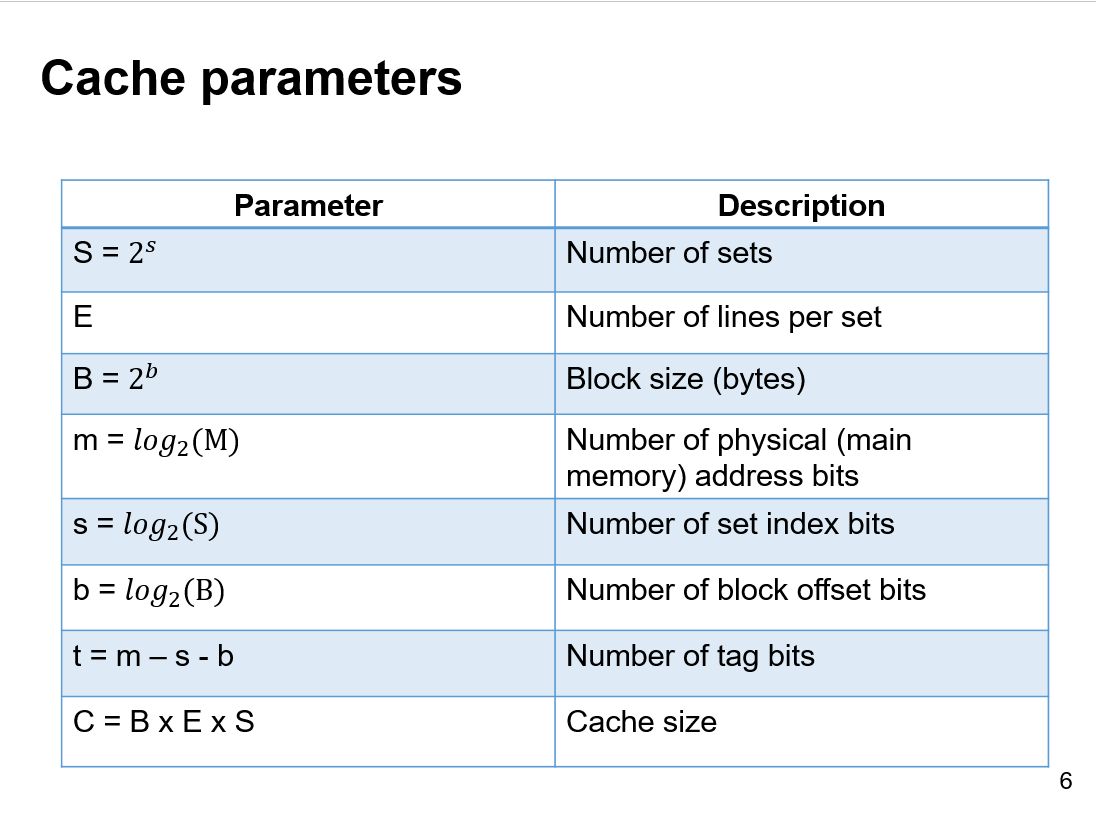
\includegraphics[width=\linewidth]{images/thetruth1.png}
  \caption{}
  \label{}
\end{figure}

\begin{figure}[h!]
  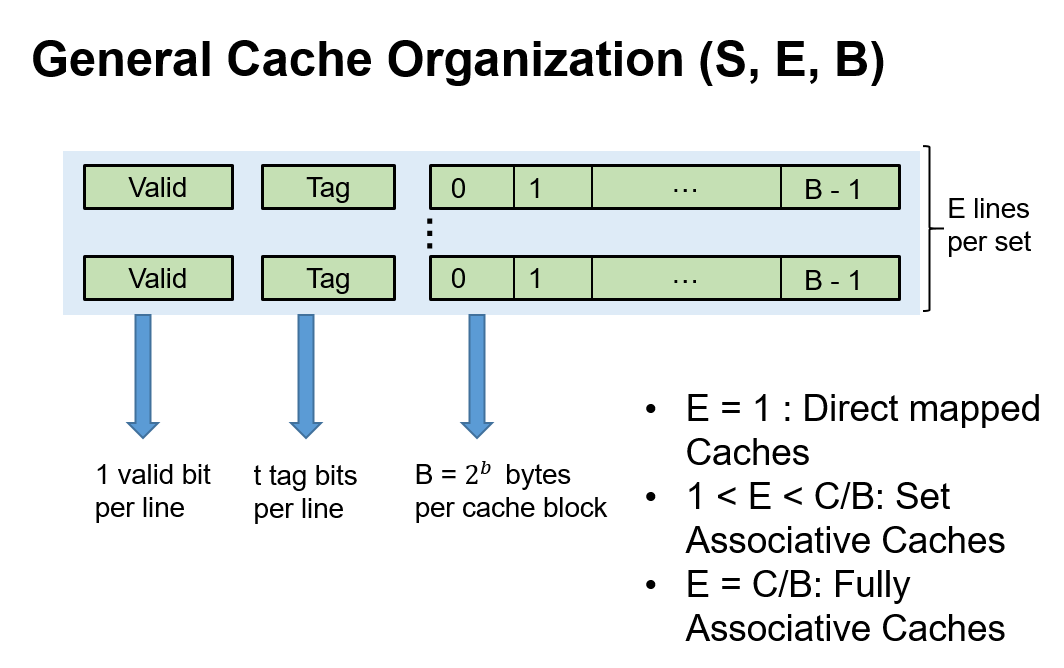
\includegraphics[width=\linewidth]{images/thetruth2.png}
  \caption{}
  \label{}
\end{figure}

\begin{figure}[h!]
  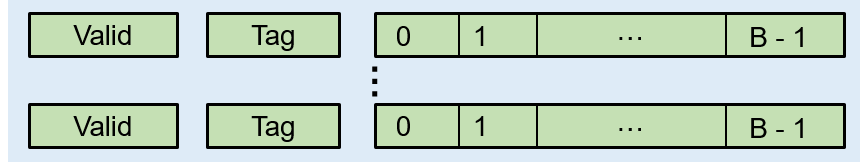
\includegraphics[width=\linewidth]{images/thetruth3.png}
  \caption{}
  \label{}
\end{figure}


\begin{figure}[h!]
  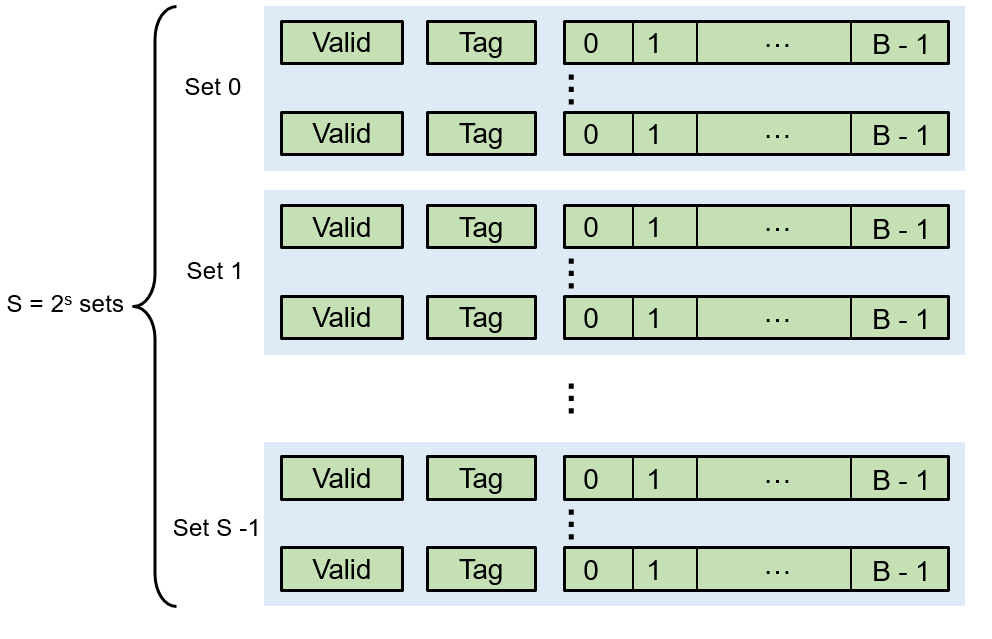
\includegraphics[width=\linewidth]{images/thetruth4.png}
  \caption{}
  \label{}
\end{figure}

\begin{figure}[h!]
  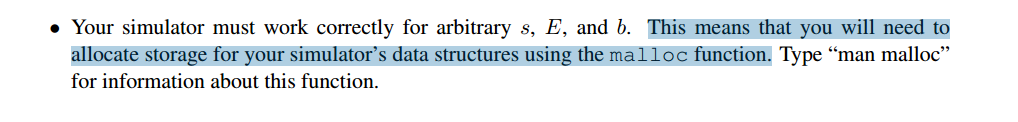
\includegraphics[width=\linewidth]{images/thetruth5.png}
  \caption{}
  \label{}
\end{figure}

\begin{figure}[h!]
  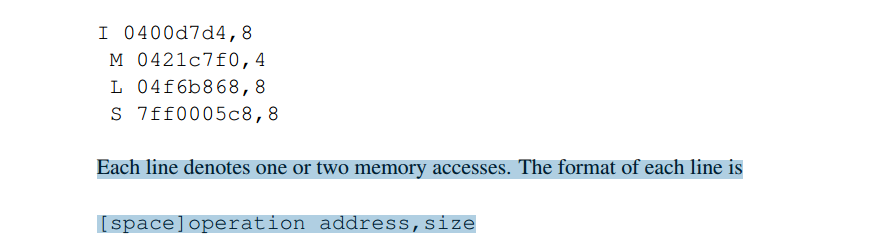
\includegraphics[width=\linewidth]{images/thetruth6.png}
  \caption{}
  \label{}
\end{figure}



\newpage
\paragraph{} 
 The first struct is cacheParameter, in which we will store all the basic information about a cache : Number of sets, Number of lines per set, Block size, Number of set index bits, Number of block offset bits. Plus, data about times that a cached is hit, missed or evicted is also stored here.



\paragraph{} 
The second struct is setLine. This represents all data in a set line in a cache. As we all knew from the slides, a set line includes a valid bit, a tag bit, and the block. For the tag bit, we declare it with the custom-defined type memoryAddress. Because this is 64 bit, it would be very annoying to keep repeating the data type declaration  Also, because we will surely deal with eviction, it is necessary to maintain a variable called last\_used to properly evict the right block later. 

\paragraph{} 
 The third struct cacheSet actually consists of a pointer to the second struct, because there are many lines of sets in a cache.  




\paragraph{} 
 The fourth struct cache actually consists of a pointer to the third struct, obviously because there are many sets in a cache. 

\paragraph{} 
After we defined all the struct needed, we will begin by building a cache. For this, we will build a function that takes in 3 parameters : number of sets, number of lines and size of the block. With these parameters, as we just loop through every line in every set and put the default value 0 inside every slot. Then we return the newly built cache. 



\paragraph{} 
Because C doesnt automatically collect the garbage for us, we also need to build a clear function due to the use of pointers in cache and cacheSet structs. We need to loop again, through all lines of all sets of a cache and free everything. 



\paragraph{} 
When we put data into the cache, first thing we need to check is whether the line that is matched is empty or not. To serve our purpose, a function to detect the empty line needs to be constructed. This function's parameters are required to supply all the  general cache parameter and one exact cache set it is checking for empty line. It shall check on only one cache set to see whether the lines inside are available or not. If all lines are unavailable, we will return -1, if there is some lines available, we will return the index of that line. 



\paragraph{} 
No line available will put us in a situation of eviction. However, choosing a line for eviction is not easy so we need another function to handle that. This function detect the right line to force eviction. Basically, we need to passed in the same 
parameters as the detect empty line function. However, that is not enough because if the next time we met eviction case, we would forget how the usage frequency of the line was. That is dangerous because we cannot decide which one is the latest-used one. Therefore, we need an array that stored 2 values : one is the line that is latest-used line and another is the oldest-used (least-recently-used) line. And notice that the pdf file requires us to "This means that you will need to allocate storage for your simulator’s data structures using the malloc function." Thanks to stackoverflow i know how to make a dynamic array in C. (http://stackoverflow.com/questions/12675919/dynamic-array-in-c-is-my-understanding-of-malloc-realloc-correct)If the cache is full, overwrite should be done to the least-recently-used line.  This function should return the index of the least-recently-used line.   


\paragraph{} 
One of the most important part of our program is the function that actually run to check if the cache is hit/missed/evicted. Here I call that function testCacheFunction and pass in the cache, the cache parameter as well as the address for it to finish its job. In this function, first we need to find the tag size ( using equation tagsize = m-s-b). After that, we need to extract the input tag bit from the address. Moreover, we need to store it in the unsigned long long because the shifting may cause negative value to appear. Plus, we also need to extract the index of the set so that we can find the exact place to put the bits.  

\paragraph{} 
Now, simply loop through the line in the sets and check the valid tag. If the valid tag is different from 0 and the input tag matches that line tag, then it is safe for us to raise the hit because we did "cache hit". Also, we need to raise the latest used variable and update the exampleSet.lines because we are working mainly on exampleSet. If we found an empty line then simply reset the checkFullCache to 0 to know that the cache was not full.  

\paragraph{} 
When the loop is done, we knew about the "cache hit". But how about "cache miss". It is very simple. We just confirm if the default hit value that we initiate with the struct cacheParameter is equal to the hit value that we got after the loop. Equality means no "cache hit" was done. No "cache hit" means "cache miss" and we need to write the data into the cache ourself. Here comes the momment that we check if the cache is full or not. If it is full then eviction should be done and for eviction to be applied properly, we need to used detectEvictLine that we wrote above. When the cache is full, we overwrite to the line that is least-recently touched. If the cache is not full, we will write our data to another empty line and remember to raise the valid bit as well as the latestUsed variable. Keeping track of all these things is very important because our traces got a lot of cache accesses to be checked, not one. 

\begin{figure}[h!]
  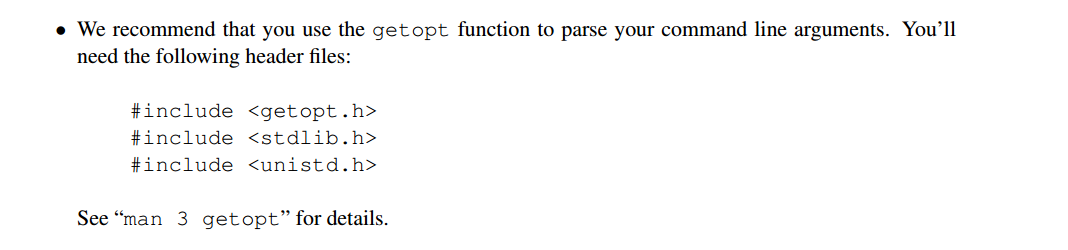
\includegraphics[width=\linewidth]{images/thetruth8.png}
  \caption{}
  \label{}
\end{figure}
\paragraph{} 
In our main program, we should figure out a way to take in parameters from command line as well as take in cache accessed from the trace files. Reading the pdf file, they suggest  we use getopt.h . After google searching, I apply the same syntax found here (https://www.gnu.org/software/libc/manual/html\_node/Example-of-Getopt.html) and here ( https://www.gnu.org/software/libc/manual/html\_node/Using-Getopt.html ) and convert string to integet (http://www.cplusplus.com/reference/cstdlib/atoi/) was able to take out s E b t g from command line. For reading file I follow instruction and example from here (https://www.tutorialspoint.com/cprogramming/c\_file\_io.htm) . Of course, we also have to take in command in tracefile because each case needs to be handled differently, especially M case needs double time.

\paragraph{} 
Some additional function was used during the process of finishing this like bzero (http://pubs.opengroup.org/onlinepubs/009695399/functions/bzero.html) to initiate the struct example Parameter ( it's like a constructor for a class in C++ but I cannot find a way to play construtor in C ).



\newpage
\section{Part B}

\paragraph{}
We need to  write a transpose function in trans.c that causes as few cache misses as possible. For every size (32x32, 64x64, 61x67), first we need to choose the block size and then apply blocking to minimize the misses.
Some important info is that  s=5, E=1, b=5 , which means we have 32 sets, direct-mapped, 32 bytes per block.  
In the first case (32 x 32) we choose block size 8. We choose it because the cache can hold a entirely 8x8 block of data in this case . In another word, accessing the data within a 8x8 block will only cause cold misses. Therefore, we can divide the 32x32 matrix into 16 blocks with the size of 32x32, and transpose block by block. All the process is done through 2 loops. However, it is notable that if the row number is equal to the column number, it means we touched the diagonal position of the square. Now we need to take care that we are accessing A and B in the same innerloop, and A, B have differnt tags. For the diagonal blocks, there are conflicts when accessing the same row of A and B. This part should not be moved or reassigned to avoid misses. Instead, we used 2 temporary variable, 1 to store the position, 1 to store the value for later assign.  use temporary local variables to avoid having to re-access those elements. For the third case ( 61 x 67 ), the method is actually the same. Moreover, when testing block size, it shows that it can run with bigger block size equals to 16. The problem with this case is that 61 x 67 doesnt form a square. So by using loops as case 32 x 32 to do transpose and minimize misses, we may get out of range and this will results in invalid access. Therefore, the condition inside the inner loop must also check if we are accessing the right place or not and limit us in the safe zone. With that being done, this case is solved.
\paragraph{}
The hardest case is 64 x 64. Because it is very hard I make a separate transpose function for it. With this function, it can utilizes fully 12 variables allowed to be declared without having to share these variables with two other cases. First of all, we declare some variables that are needed for this case. Here we choose block size 8 for optimization. We declare a bunch of single variables (which is actually equals to a 8-sized array, but not constructed as an array) , all serve as temporary data for our transpose function. 
\paragraph{}
Each time we read in a 8x8 block. Then inside, we first operate on a 4x8 block. The first loop goes through a 4 collumn 8 row of A. In this loop we  use the supporting variables to store all elements of a row. Then we try to transpose with the right positions in B. However, we are doing on a 4 row x 8 collumn B to avoid cache miss so not all elements will be transposed correctly. For example A[3][5] cannot be transposed to B[5][3]. Thus, such elements which can't be transposed correctly will be stored in another location for later use. In the code, I comment "Good job" for the elements that are transposed correctly. "Later use" for later assignment. Now that we have dealt with the first 4 col 8 arrow of A. The next job to deal with the "later use" assignment above. The "later use" assignments that we did above have taken a lot of places, so we need to bring these elements to their right positions using all the supporting variables, while still minimizing cache miss by only accesing 2 rows of A, 2 collums of B. The loop after this deals with the remaining elements.

\newpage





\clearpage



\end{document}






